\documentclass[conference]{../cls/IEEEtran}

\usepackage{graphicx}

\begin{document}

\title{Behavior Estimation on Energy-Efficient Urban Traffic Control to Explore
Operational Feasibility}

\author{
	\IEEEauthorblockN{Dominik Ascher}
	\IEEEauthorblockA{
		Chair IV: Software \& Systems Engineering\\
		Technische Universit\"at M\"unchen\\
		Boltzmannstr.\ 3, 85748 Garching, Germany\\
		Email: ds.ascher@gmail.com
	}
	\and
	\IEEEauthorblockN{Georg Hackenberg}
	\IEEEauthorblockA{
		Chair IV: Software \& Systems Engineering\\
		Technische Universit\"at M\"unchen\\
		Boltzmannstr.\ 3, 85748 Garching, Germany\\
		Email: hackenbe@in.tum.de
	}
}

\maketitle

\begin{abstract}
Many application ideas arise from increasing computational and communicational capabilities of today's automotive vehicles.
Early studies are needed to show the feasibility and potential of these ideas to foster future research and development.
\end{abstract}

\begin{IEEEkeywords}
Feasibility study, urban traffic control, eco-routing.
\end{IEEEkeywords}

\section{Motivation}

\textit{State of the art: Urban traffic control (cooperative), agent-based
approaches, congestion management.}

In the recent decades, Urban Traffic Control (UTC) has seen (a multitude of)
approaches dealing with the complexity of action and interaction between
multiple traffic participants through elaborate control systems. 
In this context, (a large number of) approaches incorporating
(multi-)agent systems have shown to be effective and have established
agent systems as a pervasive paradigm ~\cite{Chen2010},~\cite{Roozemond1999}.

Coordination and interaction between several agents are a complex problem.
In common UTC approaches, the focus lies within optimizing traffic control
agents, e.g.
regulating traffic lights, while agents representing vehicles are frequently used to promote and communicate information
within the system. Major problem of these approaches is to avoid traffic
congestion, while coordinating a multitude of vehicles.

The majority of approaches focuses on the optimization of traffic control
system regulation methods, while less research effort is put
on the behavior of individual vehicles and their underlying control logic. 

Dresner and Stone ~\cite{Dresner2008} discuss a novelty multi-agent approach of
intersection management with autonomous vehicles interacting among themselves using artificial
intellience. Through the interaction between intelligent and autonomous
vehicles, conventional methods of vehicle coordination between human drivers like traffic lights and 
stops signs are no longer necessary, resulting in more efficient
vehicle behavior through reduced waiting times and congestion susceptibility.


\textit{Transition to Second direction: Eco-routing (energy efficient, fast, but
not cooperative).}

In this paper, Eco-Routing refers to the concept of selecting the most
energy-efficient route between two locations.
\textit{+Differing Definitions : ShortestPath + EnergyOptimization Problem}
Frequent mentions refer the origin of the term Eco-Routing to
~\cite{Barth2007}, who proposes a environmentally-friendly
navigation technique towards Intelligent Transportation Systems (ITS).

\textit{+Handling of congestions, most-energy-efficient route possibly
subject to congestion}

 ~\cite{Boriboonsomsin2012} introduced a (reactive) eco-routing (navigation)
 system alleviating the problem of congestion through the
 incorporation of historical and real-time traffic information for individual
 traffic participants.


\textit{Energy-efficient urban traffic control approaches are
missing, i.e.
the combination of urban traffic control and eco-routing.}

In summary, eco-routing approaches offer efficient routing techniques, which
concentrate on the energy-efficient routing of single traffic participants in
relation to their current environment.  In contrast, UTC approaches utilize the
cooperation and interaction between multiple traffic participants for congestion
management within well-defined boundaries, i.e.
cities. 
However, while the current approaches of both
directions offer feasible techniques/solutions towards specific problems, they are
subject to their limited scope and do not consider an holistic integration of
congestion management with energy-efficient routing (eco-routing). Therefore,
current UTC approaches remain unaligned towards energy-efficient vehicle
behavior and minimization of emissions.

To overcome this situation, in this paper, we report on first steps towards an
operational feasibility study of energy-efficient urban traffic control.
In the following we shortly describe the underlying behavior estimation
framework before explaining the energy-efficient urban traffic control demonstrator as well as initial performance analysis results.

\section{Behavior Estimation Framework}

To illustrate the scope of our work we first give a short definition of feasibility studies: 
According to Whitten et al.~\cite{Whitten2005} in systems engineering feasibility studies follow the requirements discovery phase to uncover potential opportunities and threads.
Upon successful feasibility demonstration the system design, implementation and operation phases follow.

\begin{figure}[b]
	\centering
	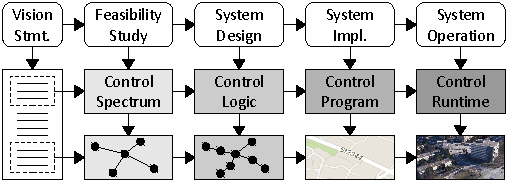
\includegraphics{../gfx/process.pdf}
	\caption{Overview of the general systems engineering process from requirements discovery over feasibility study, system design and implementation to system operation adapted to cooperative eco-routing.}
	\label{figure:process}
\end{figure}
We translate this process to cooperative eco-routing as illustrated in Figure~\ref{figure:process}.
Given the requirements (i.e.\ energy-efficient and congestion-free routing) we develop a control spectrum specification and analyze it with respect to an approximate physical model.
Technically, we base our work on early emergent property estimation techniques described in~\cite{Hackenberg2012}.
Consequently, we use a discrete-time and continuous-state system model as depicted in Figure~\ref{figure:framework}.
We rely on discrete-time models to reduce the reachable state space during analysis.
However, we use continuous-state models because quantities like velocity or distance can be described more intuitively.
Moreover, we rely on a generic and reusable model architecture dividing the system into software, context, constraint, objective and equivalence components.
In particular, the partial software model describes the control spectrum, while the context model describes the physical state.
Based on the physical state the constraint and objective models define the operational limits and goals.
Finally, the equivalence model describes how the physical states can be clustered during state space exploration.
Behavior estimation uses stochastic optimization techniques similar to~\cite{Pereira1991} to approximate optimal system behavior.

\begin{figure}[b]
	\centering
	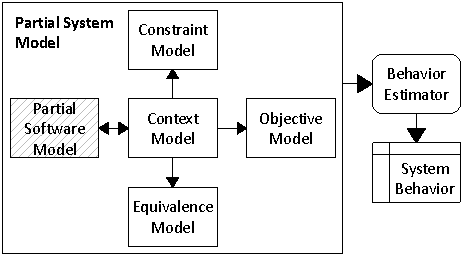
\includegraphics{../gfx/framework.pdf}
	\caption{Overview of the estimation framework including component-based system model (including non-deterministic software component), behavior estimator and system behavior.}
	\label{figure:framework}
\end{figure}

\section{Energy-Efficient Urban Traffic Control}

Model architecture: Context (i.e.\ vehicle) component, constraint component, objective component, control component, equivalence component.
For the presented approach, components are based on the presented models
accordingly.

Component behavior: Speed selection, edge selection, edge-based collision detection, energy consumption, etc.

The behavior of the context component, i.e. vehicle component, is defined by
it's edge, relative position on the edge, speed and according energy
consumption.

Edge selection is based on the available choices on the current position of the
vehicle. For traversing a given edge, vehicles have to completely cross their
selected edge. If a vehicle has crossed an edge, it is able to (randomly)
select a new edge to travel to. 

Vehicle speed selection depends on a continous value range.
From this range of values, a (random) value is drawn. Speed selection is
instantaneous, which has shown to provide appropriately accurate results in
comparable mescoscopic approaches [?].

Energy consumption is determined via the vehicles edge and speed. The edge determines the altitude difference between the edges source and
target, while the speed has an quadratic relationship to observed energy
consumption. (in accordance to study observation results[?])

Driving behavior is derived from objectives, which are formulated as cost
functions. Cost function A measures the elapsed time since the start of the
simulation until the target has been reached. Cost function B
determines the vehicles current energy consumption in relation to the
vehicles maximum possible energy consumption. Different weighting of cost
functions can be applied, resulting in accordingly adjusted vehicle driving
behavior. Furthermore, in environments with multiple vehicles, different
priorities of vehicles in the traffic system can be introduced through
differently weighting individual vehicle costs.

The behavior of multiple vehicles is prone to collisions in case their relative
positions on edges are not checked against. Collision detection between
multiple vehicles is performed via a collision constraint. The constraint tests
for every pair of active vehicles whether the sum of their currently selected
relative position on the edge and half the vehicles length overlap/match
partially.
If that is the case, it tests wether the difference in their respective position 
is greater than the combined length of the pair of currently observed vehicles. 
If this doesn't apply, the constraint
tests whether there are free lanes available on the current position based on
edge capacity, i.e. the number of lanes of a given road segment. Therefore, the
test's outcome depends on the unoccupied lanes available at the relative
position on the edge.

Behavior estimation: One basic case (single vehicle, two routes) and one more complex case (multiple vehicles).
To estimate the behavior of the approach, we demonstrate a basic case of a
single vehicle within a traffic system featuring two routes with similar
starting points and targets varying in their respective energy-efficiency. While
route A represents a flat route profile, route B offers a route profile with differing heights, but, compared to route A,
shorter distance to target. : Simulation results.

In a second case, we compare how well our control approach copes with a
multitude of vehicles and a bigger traffic network. : Simulation results.

\section{Conclusion and Outlook}

We presented behavior estimation results of a new approach for Urban Traffic
Control utilizing a energy-efficient and autonomous vehicle control strategy.

Great stuff! :)

\bibliographystyle{../bst/IEEEtran}
\bibliography{ICCVE-2014}

\end{document}
